\documentclass[12pt]{article}
\usepackage{amssymb,mathrsfs, amsmath,amsfonts}
\usepackage{mathtools}
\usepackage{graphicx}
\usepackage{enumitem}
\usepackage{braket}
\graphicspath{ {./ps1-assets/}{./exercises/handwritten/ps1-assets/} }

\title{Problem Set 1 Solutions}
\author{CSE 468}
\date{\today}

\begin{document}

\maketitle

\noindent \textbf{Note:} Many of these problems use  https://lab.quantumflytrap.com/lab.

\begin{enumerate}[font=\bfseries]
    \item \begin{enumerate}
        \item \[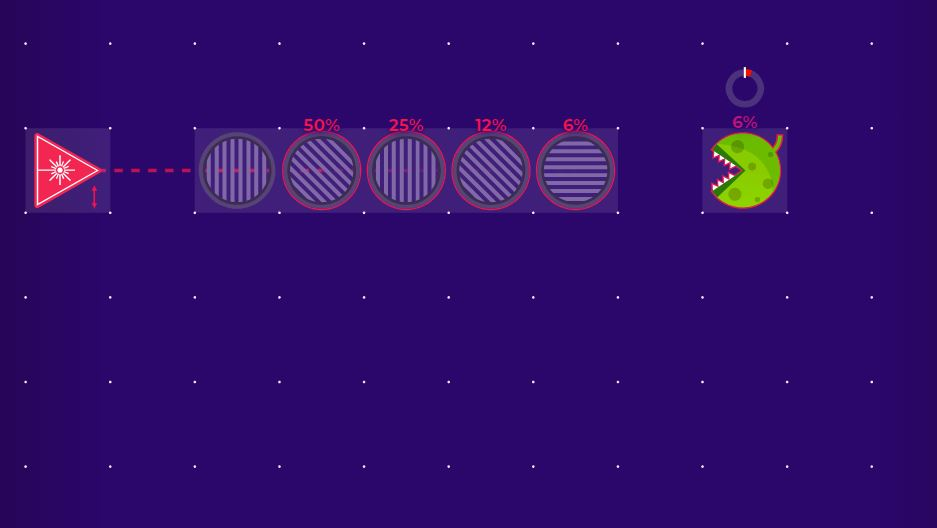
\includegraphics[scale=0.6]{easyFilter-sol}\]
        \item Use a sequence of k filters with the initial filter rotated 45 degrees relative to the photon source and then rotate each additional filter by another 45 degrees.
        \item \begin{pmatrix}
                0 & 0 \\
                0 & 1
                \end{pmatrix}
        \item $\sin^2{\theta}$
        \item \begin{pmatrix}
                \cos^2{\theta} & \cos{\theta}\sin{\theta} \\
                \sin{\theta}\cos{\theta} & \sin^2{\theta}
                \end{pmatrix}
        \item Begin with a photon oriented completely in the vertical direction so we have $\begin{pmatrix} 0 \\ 1 \end{pmatrix}$. We then apply a filter oriented 45 degrees ($\frac{\pi}{4}$ radians) from the x-axis. This is represented by the following operation:
        \[\begin{pmatrix}
                \cos^2{(\frac{\pi}{4})} & \cos{(\frac{\pi}{4})}\sin{(\frac{\pi}{4})} \\
                \sin{(\frac{\pi}{4})}\cos{(\frac{\pi}{4})} & \sin^2{(\frac{\pi}{4})}
                \end{pmatrix}
                \begin{pmatrix} 0 \\ 1 \end{pmatrix}
                = 
                \begin{pmatrix}
                \frac{1}{2} & \frac{1}{2} \\
                \frac{1}{2} & \frac{1}{2}
                \end{pmatrix}
                \begin{pmatrix} 0 \\ 1 \end{pmatrix}
                =
                \begin{pmatrix} \frac{1}{2} \\ \frac{1}{2} \end{pmatrix}
                \]
            Note the norm of this vector is $\frac{1}{2}$ (half of the light is absorbed by the filter). We next apply a vertically oriented filter and obtain
            \[\begin{pmatrix}
                0 & 0 \\
                0 & 1
                \end{pmatrix}
                \begin{pmatrix}
                \frac{1}{2} \\ \frac{1}{2}
                \end{pmatrix}
                =
                \begin{pmatrix} 0 \\ \frac{1}{2} \end{pmatrix}
                \]
            Continue in a similar manner for the last 2 filters.
            \item No. Applying a vertical filter followed by a horizontal filter absorbs all the light. Applying a vertical filter, then a filter oriented 45 degrees from the origin, and then a horizontal filter will let $\frac{1}{8}$ of the original light through. Note this question depends on what polarization we assume the photon source admits. 
    \end{enumerate}
    \item \begin{enumerate}
        \item \[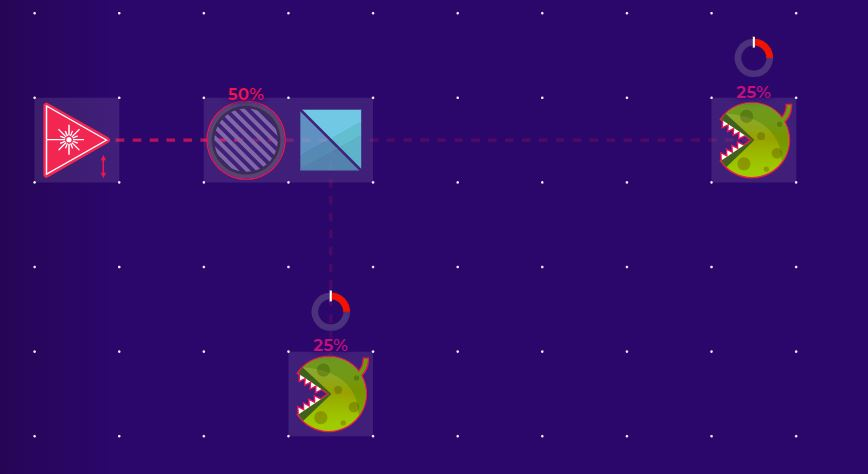
\includegraphics[scale=0.6]{beamSplit-sol}\]
        \item The maximum probability of a photon arriving at receiver A or receiver B is 50\% because we must use a polarizing filter to rotate the photons by 45 degrees to effectively use the polarizing beam splitter. This first filter allows 50\% of the original photons through, so the maximum percentage possible is 50\%.
    \end{enumerate}
    \item \begin{enumerate}
        \item \[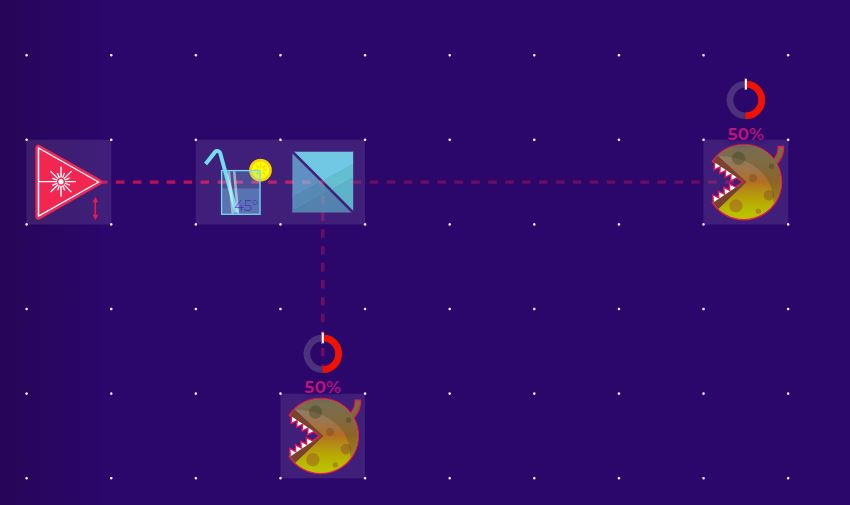
\includegraphics[scale=0.6]{sugarSplit-sol}\]
        \item The maximum possible probability of a photon arriving at receiver A or receiver B is now 100\% because we can use the sugar solution to rotate photons by 45 degrees without losing any photons like we had to do when only using polarizing filters.
    \end{enumerate}
    \item \begin{enumerate}
        \item We should expect to see a perfect 50/50 split.
        \item When I ran this experiment I observed a 51/49 split. The results do not match our expectations because quantum systems are random and noisy. We expect a perfect 50/50 split in the infinite limit.
    \end{enumerate}
    \item \[\cos^2({10^{\circ}}) \approx .97 \]
            \[(.97)^x = 0.5\]
            \[x = 22.75\]
            Should round down to 22 filters but also accept 23 filters.
\end{enumerate}



\end{document}
